\documentclass{article}
\usepackage{amssymb, amsthm, enumitem}
% Prevent file encoding error
\usepackage[utf8]{inputenc}
% Margin for viewing/printing aesthetics
\usepackage[margin=1in,top=0.5in,bottom=0.5in]{geometry}
% Stick to the left (question number) for all math equations
\usepackage[fleqn]{amsmath}
% Supposed to make the text look better (subjective) via reduced space between letters
% https://www.khirevich.com/latex/microtype/
\usepackage{microtype}
% For \begin{comment}...\end{comment}
\usepackage{verbatim}
% For syntax highlighting
\usepackage{minted}
\begin{comment}
Install: pip install Pygments
Add "-shell-escape", to vscode:
Open settings, search for "latex-workshop.latex.tools", click "Edit in settings.json", add "-shell-escape" to the pdflatex
command.
\end{comment}

% For displaying accurate time
\usepackage{datetime}
% For PDF metadata
\usepackage[pdfusetitle]{hyperref}
% For PDF outline (table of contents)
\usepackage{navigator}
% Automatically add section to outline
\newcommand{\mysectionstar}[2][]{%
    \ifthenelse{\equal{#1}{}}%
        {\section*{#2}}% If optional argument is empty
        {\section*[#1]{#2}}% If optional argument is not empty
    \outline{1}{#2}%
}
\newcommand{\mysubsectionstar}[2][]{%
    \ifthenelse{\equal{#1}{}}%
        {\subsection*{#2}}% If optional argument is empty
        {\subsection*[#1]{#2}}% If optional argument is not empty
    \outline{2}{#2}%
}
\newcommand{\mysubsubsectionstar}[2][]{%
    \ifthenelse{\equal{#1}{}}%
        {\subsubsection*{#2}}% If optional argument is empty
        {\subsubsection*[#1]{#2}}% If optional argument is not empty
    \outline{3}{#2}%
}
% For images
\usepackage{graphicx}
\begin{comment}
Usage:
\begin{figure}[H]
\centering
\includegraphics[width=0.4\textwidth]{image.png}
\caption{Descriptive text for Figure}
\end{figure}
\end{comment}
% For pseudocode
\usepackage{algorithm}
\usepackage{algpseudocode}
% For scalable fonts
\usepackage{lmodern}
% For graph
\usepackage{pgfplots}
\pgfplotsset{compat=1.18}

% Independent symbol
\newcommand\independent{\protect\mathpalette{\protect\independenT}{\perp}}
\def\independenT#1#2{\mathrel{\rlap{$#1#2$}\mkern2mu{#1#2}}}

\title{STAT2602 Assignment 4}
\author{Cheng Ho Ming, Eric (3036216734) [Section 1A, 2024]}
\date{\today \ \currenttime}

\begin{document}
\maketitle

\mysectionstar{Q1}
Let $X_1, X_2, \cdots, X_n$ and $Y_1, Y_2, \cdots, Y_m$ be random samples from distributions $N(\theta_1, \theta_3)$ and $N(\theta_2, \theta_4)$, respectively. Assume that $X_1, X_2, \cdots, X_n$, $Y_1, Y_2, \cdots, Y_m$ are independent. \\
Find the generalized likelihood ratio test statistic for hypotheses:
\[ H_0 : \theta_1 = \theta_2 \text{ and } \theta_3 = \theta_4 \quad \text{versus} \quad H_1 : \theta_1 \neq \theta_2 \text{ or } \theta_3 \neq \theta_4. \]

$\newline$
The likelihood function under $H_0 \cup H_1$ is:
\[
L(\theta_1, \theta_2, \theta_3, \theta_4) = \prod_{i=1}^n \frac{1}{\sqrt{2\pi\theta_3}} \exp\left( -\frac{(X_i - \theta_1)^2}{2\theta_3} \right) \times \prod_{j=1}^m \frac{1}{\sqrt{2\pi\theta_4}} \exp\left( -\frac{(Y_j - \theta_2)^2}{2\theta_4} \right)
\]
The log-likelihood function is given by:
\[
\ell(\theta_1, \theta_2, \theta_3, \theta_4) = -\frac{n}{2} \ln(2\pi\theta_3) - \frac{1}{2\theta_3} \sum_{i=1}^n (X_i - \theta_1)^2 - \frac{m}{2} \ln(2\pi\theta_4) - \frac{1}{2\theta_4} \sum_{j=1}^m (Y_j - \theta_2)^2
\]
To find the MLEs, we take partial derivatives with respect to each parameter and set them to zero.
\begin{minipage}{.5\linewidth}
$\newline$
The MLE of $\theta_1$ under $H_0 \cup H_1$ is:
\begin{align*}
\frac{\partial \ell}{\partial \theta_1} &= 0 \\
\frac{1}{\theta_3} \sum_{i=1}^n (X_i - \theta_1) &= 0 \\
\sum_{i=1}^n (X_i - \theta_1) &= 0 \\
n\theta_1 &= \sum_{i=1}^n X_i \\
\hat{\theta}_1 &= \frac{1}{n} \sum_{i=1}^n X_i = \bar{X}
\end{align*}
\end{minipage}
\begin{minipage}{.5\linewidth}
$\newline$
The MLE of $\theta_2$ under $H_0 \cup H_1$ is:
\begin{align*}
\frac{\partial \ell}{\partial \theta_2} &= 0 \\
\frac{1}{\theta_4} \sum_{j=1}^m (Y_j - \theta_2) &= 0 \\
\sum_{j=1}^m (Y_j - \theta_2) &= 0 \\
m\theta_2 &= \sum_{j=1}^m Y_j \\
\hat{\theta}_2 &= \frac{1}{m} \sum_{j=1}^m Y_j = \bar{Y}
\end{align*}
\end{minipage}
\begin{minipage}{.5\linewidth}
$\newline$
The MLE of $\theta_3$ under $H_0 \cup H_1$ is:
\begin{align*}
\frac{\partial \ell}{\partial \theta_3} &= 0 \\
-\frac{n}{2\theta_3} + \frac{1}{2\theta_3^2} \sum_{i=1}^n (X_i - \theta_1)^2 &= 0 \\
-\frac{n}{\theta_3} + \frac{1}{\theta_3^2} \sum_{i=1}^n (X_i - \theta_1)^2 &= 0 \\
\frac{1}{\theta_3^2} \sum_{i=1}^n (X_i - \theta_1)^2 &= \frac{n}{\theta_3} \\
\theta_3 &= \frac{1}{n} \sum_{i=1}^n (X_i - \theta_1)^2
\end{align*}
Substituting \( \hat{\theta}_1 = \bar{X} \):
\[
\hat{\theta}_3 = \frac{1}{n} \sum_{i=1}^n (X_i - \bar{X})^2
\]
\end{minipage}
\begin{minipage}{.5\linewidth}
$\newline$
The MLE of $\theta_4$ under $H_0 \cup H_1$ is:
\begin{align*}
\frac{\partial \ell}{\partial \theta_4} &= 0 \\
-\frac{m}{2\theta_4} + \frac{1}{2\theta_4^2} \sum_{j=1}^m (Y_j - \theta_2)^2 &= 0 \\
-\frac{m}{\theta_4} + \frac{1}{\theta_4^2} \sum_{j=1}^m (Y_j - \theta_2)^2 &= 0 \\
\frac{1}{\theta_4^2} \sum_{j=1}^m (Y_j - \theta_2)^2 &= \frac{m}{\theta_4} \\
\theta_4 &= \frac{1}{m} \sum_{j=1}^m (Y_j - \theta_2)^2
\end{align*}
Substituting \( \hat{\theta}_2 = \bar{Y} \):
\[
\hat{\theta}_4 = \frac{1}{m} \sum_{j=1}^m (Y_j - \bar{Y})^2
\]
\end{minipage}
$\therefore$ Under $H_0 \cup H_1$, the likelihood function is:
\begin{align*}
\ell(\theta_1, \theta_2, \theta_3, \theta_4) &= -\frac{n}{2} \ln(2\pi\theta_3) - \frac{1}{2\theta_3} \sum_{i=1}^n (X_i - \theta_1)^2 - \frac{m}{2} \ln(2\pi\theta_4) - \frac{1}{2\theta_4} \sum_{j=1}^m (Y_j - \theta_2)^2 \\
&= -\frac{n}{2} \ln(2\pi\hat{\theta}_3) - \frac{n}{2} - \frac{m}{2} \ln(2\pi\hat{\theta}_4) - \frac{m}{2}
\end{align*}

$\newline$
Under the null hypothesis \( H_0 \), we let $\theta_1 = \theta_2 = \theta$ and $\theta_3 = \theta_4 = \theta_v$. \\
The likelihood function is:
\[
L_0(\theta, \theta_v) = \prod_{i=1}^n \frac{1}{\sqrt{2\pi\theta_v}} \exp\left( -\frac{(X_i - \theta)^2}{2\theta_v} \right) \times \prod_{j=1}^m \frac{1}{\sqrt{2\pi\theta_v}} \exp\left( -\frac{(Y_j - \theta)^2}{2\theta_v} \right)
\]
The log-likelihood function is:
\[
\ell_0(\theta, \theta_v) = -\frac{n+m}{2} \ln(2\pi\theta_v) - \frac{1}{2\theta_v} \left( \sum_{i=1}^n (X_i - \theta)^2 + \sum_{j=1}^m (Y_j - \theta)^2 \right)
\]
The MLE of $\theta_1 = \theta_2 = \theta$ under $H_0$ is:
\begin{align*}
\frac{\partial \ell_0}{\partial \theta} &= 0 \\
-\frac{1}{2\theta_v} \left( -2 \sum_{i=1}^n (X_i - \theta) - 2 \sum_{j=1}^m (Y_j - \theta) \right) &= 0 \\
\frac{1}{\theta_v} \left( \sum_{i=1}^n (X_i - \theta) + \sum_{j=1}^m (Y_j - \theta) \right) &= 0 \\
\sum_{i=1}^n X_i - n\theta + \sum_{j=1}^m Y_j - m\theta &= 0 \\
(n + m)\theta &= \sum_{i=1}^n X_i + \sum_{j=1}^m Y_j \\
\hat{\theta} &= \frac{1}{n + m} \left( \sum_{i=1}^n X_i + \sum_{j=1}^m Y_j \right) \\
&= \frac{n\bar{X} + m\bar{Y}}{n + m}
\end{align*}
The MLE of $\theta_3 = \theta_4 = \theta_v$ under $H_0$ is:
\begin{align*}
\frac{\partial \ell_0}{\partial \theta_v} &= 0 \\
-\frac{n+m}{2\theta_v} + \frac{1}{2\theta_v^2} \left( \sum_{i=1}^n (X_i - \theta)^2 + \sum_{j=1}^m (Y_j - \theta)^2 \right) &= 0 \\
-\frac{n+m}{\theta_v} + \frac{1}{\theta_v^2} \left( \sum_{i=1}^n (X_i - \theta)^2 + \sum_{j=1}^m (Y_j - \theta)^2 \right) &= 0 \\
\frac{1}{\theta_v^2} \left( \sum_{i=1}^n (X_i - \theta)^2 + \sum_{j=1}^m (Y_j - \theta)^2 \right) &= \frac{n+m}{\theta_v} \\
\theta_v &= \frac{1}{n + m} \left( \sum_{i=1}^n (X_i - \theta)^2 + \sum_{j=1}^m (Y_j - \theta)^2 \right)
\end{align*}
Substituting \( \hat{\theta} = \frac{n\bar{X} + m\bar{Y}}{n + m} \):
\[
\hat{\theta}_v = \frac{1}{n + m} \left( \sum_{i=1}^n (X_i - \hat{\theta})^2 + \sum_{j=1}^m (Y_j - \hat{\theta})^2 \right)
\]
$\therefore$ Under $H_0$, the likelihood function is:
\begin{align*}
\ell_0(\theta, \theta_v) &= -\frac{n+m}{2} \ln(2\pi\theta_v) - \frac{1}{2\theta_v} \left( \sum_{i=1}^n (X_i - \theta)^2 + \sum_{j=1}^m (Y_j - \theta)^2 \right) \\
&= -\frac{n+m}{2} \ln(2\pi\hat{\theta}_v) - \frac{n + m}{2}
\end{align*}
The generalized likelihood ratio is:
\[
\Lambda = \frac{\underset{\theta \in \Theta_0}{\max} L(\theta)}{\underset{\theta \in \Theta}{\max} L(\theta)} = \frac{L_0}{L}
\]
Take natural-log of the generalized likelihood ratio to simplify the steps:
\begin{align*}
\ln \Lambda &= \ln L_0 - \ln L = \ell_0 - \ell \\
\ln \Lambda &= -\frac{n+m}{2} \ln(2\pi\hat{\theta}_v) - \frac{n + m}{2} - (-\frac{n}{2} \ln(2\pi\hat{\theta}_3) - \frac{n}{2} - \frac{m}{2} \ln(2\pi\hat{\theta}_4) - \frac{m}{2}) \\
\ln \Lambda &= -\frac{n+m}{2} \ln(2\pi\hat{\theta}_v) - \frac{n + m}{2} + \frac{n}{2} \ln(2\pi\hat{\theta}_3) + \frac{n}{2} + \frac{m}{2} \ln(2\pi\hat{\theta}_4) + \frac{m}{2} \\
\ln \Lambda &= -\frac{n+m}{2} \ln(2\pi\hat{\theta}_v) + \frac{n}{2} \ln(2\pi\hat{\theta}_3) + \frac{m}{2} \ln(2\pi\hat{\theta}_4) \\
\Lambda &= \exp\left( -\frac{n+m}{2} \ln(2\pi\hat{\theta}_v) + \frac{n}{2} \ln(2\pi\hat{\theta}_3) + \frac{m}{2} \ln(2\pi\hat{\theta}_4) \right) \\
\Lambda &= \left( 2\pi\hat{\theta}_v \right)^{\frac{n+m}{2}} \left( \frac{1}{2\pi\hat{\theta}_3} \right)^{\frac{n}{2}} \left( \frac{1}{2\pi\hat{\theta}_4} \right)^{\frac{m}{2}} \\
\Lambda &= \left( \frac{\hat{\theta}_v}{\hat{\theta}_3} \right)^{\frac{n}{2}} \left( \frac{\hat{\theta}_v}{\hat{\theta}_4} \right)^{\frac{m}{2}}
\end{align*}

$\newline$
Therefore, the generalized likelihood ratio test statistic is:
\[
\Lambda = \left( \frac{\hat{\theta}_v}{\hat{\theta}_3} \right)^{\frac{n}{2}} \left( \frac{\hat{\theta}_v}{\hat{\theta}_4} \right)^{\frac{m}{2}}
\]
for $\hat{\theta}_v = \frac{1}{n + m} \left( \sum_{i=1}^n (X_i - \hat{\theta})^2 + \sum_{j=1}^m (Y_j - \hat{\theta})^2 \right)$, $\hat{\theta}_3 = \frac{1}{n} \sum_{i=1}^n (X_i - \hat{\theta})^2$, and $\hat{\theta}_4 = \frac{1}{m} \sum_{j=1}^m (Y_j - \hat{\theta})^2$. \\
Under very general conditions, when $H_0$ is true,
\[
-2\ln \Lambda \sim_d \chi^2(2) \text{ as } n, m \to \infty.
\]

\mysectionstar{Q2}
Let $X$ be $N(\mu, 100)$.

\mysubsectionstar{(i)}
To test $H_0 : \mu = 230$ versus $H_1 : \mu > 230$, what is the rejection region specified by the generalized likelihood ratio test?

$\newline$
The restricted MLE of $\mu$ under $H_0$ is
\[
\hat{\mu}^R = 230.
\]
The unrestricted MLE under $H_0 \cup H_1$ is
\[
\hat{\mu} =
\begin{cases}
    \bar{x} & \text{if } \bar{x} > 230, \\
    230 & \text{if } \bar{x} \leq 230.
\end{cases}
\]
The likelihood function is:
\[
L(\mu) = \left( 2\pi \times 100 \right)^{-\frac{n}{2}}
\exp\left( -\frac{1}{2 \times 100} \sum_{i=1}^n (x_i - \mu)^2 \right)
\]
When $\bar{x} \leq 230$, the generalized likelihood ratio is
\[
\frac{\left( 2\pi \times 100 \right)^{-\frac{n}{2}} \exp\left( -\frac{n}{2 \times 100} \sum_{i=1}^n (x_i - 230)^2 \right)}{\left( 2\pi \times 100 \right)^{-\frac{n}{2}} \exp\left( -\frac{n}{2 \times 100} \sum_{i=1}^n (x_i - 230)^2 \right)} = 1
\]
Therefore, the generalized likelihood ratio is
\[
\Lambda = \frac{L(\hat{\mu}^R)}{L(\hat{\mu})} =
\begin{cases}
    1 & \text{if } \bar{x} \leq 230, \\
    \exp\left( \frac{\sum (x_i - \bar{x})^2 - \sum (x_i - 230)^2}{200} \right) & \text{if } \bar{x} > 230.
\end{cases}
\]
Since $Pr(\Lambda \neq k) \neq 1$ for $0 \leq k \leq 1$, $\bar{x} \leq 230$ is not acceptable. Therefore, consider $\bar{x} > 230$:
\begin{align*}
\exp\left( \frac{\sum (x_i - \bar{x})^2 - \sum (x_i - 230)^2}{200} \right) &\leq k \\
\exp\left( \frac{\sum x_i^2 - n\bar{x}^2 - \sum x_i^2 + 2 \times 230 \sum x_i - n \times 230^2}{200} \right) &\leq k \\
\frac{-n\bar{x}^2 + 2 \times 230 \times n\bar{x} - 230^2 n}{200} &\leq \ln k \\
- (\bar{x} - 230)^2 &\leq \frac{200}{n} \ln k \\
(\bar{x} - 230)^2 &\geq -\frac{200}{n} \ln k \\
\bar{x} \leq 230 - \sqrt{-\frac{200}{n} \ln k} \quad &\text{or} \quad \bar{x} \geq 230 + \sqrt{-\frac{200}{n} \ln k}.
\end{align*}
Using Neyman-Pearson Lemma, for $H_0: \bar{x} > 230$, let the rejection region be $C = \{\bar{x} > c\}$. Then,
\begin{align*}
\alpha &= P(\text{reject } H_0 \mid H_0 \text{ is true}) \\
&= P\left(\bar{x} > c \ \middle|\ \bar{x} \sim N\left(230, \frac{100}{n}\right)\right) \\
&= P\left(\frac{\bar{x} - 230}{10 / \sqrt{n}} > \frac{c - 230}{10 / \sqrt{n}} \ \middle|\ \frac{\bar{x} - 230}{10 / \sqrt{n}} \sim N(0, 1)\right) \\
&= P\left(Z > \frac{c - 230}{10 / \sqrt{n}}\right).
\end{align*}
From the standard normal distribution, $\frac{c - 230}{10 / \sqrt{n}} = Z_\alpha \Rightarrow c = 230 + Z_\alpha \frac{10}{\sqrt{n}}$. \\
As a result, the rejection region is $C = \{\bar{x} > 230 + Z_\alpha \frac{10}{\sqrt{n}}\}.$

\mysubsectionstar{(ii)}
If a random sample of $n = 16$ yielded $\bar{x} = 232.6$, is $H_0$ accepted at a significance level of $\alpha = 0.10$? What is the $p$-value?

$\newline$
The rejection region is:
\[
230 + Z_{0.10} \frac{10}{\sqrt{16}} = 230 + 1.2816 \times 2.5 = 233.204
\]
Since $\bar{X} = 232.6 \leq 233.204$, $H_0$ is accepted at a significance level of $\alpha = 0.10$. \\
The $p$-value is:
\[
P(\bar{X} > 233.204 \mid H_0: \mu = 230) = P\left(Z > \frac{233.204 - 230}{10 / \sqrt{16}}\right) = P(Z > 1.2816) = 1 - 0.8997 = 0.1003.
\]

\mysectionstar{Q3}
Let $X_1, X_2, \cdots, X_n$ be an independent random sample from $N(\mu, \sigma^2)$ with unknown mean $\mu$ and $\sigma^2$. Show the details to find the generalized likelihood ratio test for hypotheses
\[ H_0 : \mu \geq \mu_0 \quad \text{versus} \quad H_1 : \mu < \mu_0. \]

$\newline$
The likelihood function is:
\[
L(\mu, \sigma^2) = \prod_{i=1}^{n} \frac{1}{\sqrt{2\pi\sigma^2}}e^{-\frac{(X_i - \mu)^2}{2\sigma^2}}
\]
The generalized likelihood ratio is:
\[
\Lambda = \frac{L(\Omega_0)}{L(\Omega)} = \frac{\underset{\mu \geq \mu_0}{\max} L(\mu, \sigma^2)}{\underset{\mu}{\max} L(\mu, \sigma^2)} \text{ where } \Omega_0 = \{\mu \geq \mu_0\} \text{ and } \Omega = \{\mu \in \mathbb{R}\}.
\]
In order to find $\underset{\mu \geq \mu_0}{\max} L(\mu, \sigma^2)$, which is the maximum likelihood estimate of $\mu$ under the null hypothesis, we consider the log-likelihood function:
\[
\ell(\mu, \sigma^2) = \ln L(\mu, \sigma^2) = \sum_{i=1}^{n} \ln \left(\frac{1}{\sqrt{2\pi\sigma^2}}e^{-\frac{(X_i - \mu)^2}{2\sigma^2}}\right) = -\frac{n}{2} \ln(2\pi\sigma^2) - \frac{1}{2\sigma^2} \sum_{i=1}^{n} (X_i - \mu)^2
\]
Differentiating $\ell(\mu, \sigma^2)$ with respect to $\mu$:
\begin{align*}
\frac{\partial \ell}{\partial \mu} &= \sum_{i=1}^{n} \frac{\partial}{\partial \mu} \left(-\frac{(X_i - \mu)^2}{2\sigma^2}\right) \\
&= \sum_{i=1}^{n} \frac{X_i - \mu}{\sigma^2} \\
&= \frac{n(\bar{X} - \mu)}{\sigma^2}
\end{align*}
Setting $\frac{\partial \ell}{\partial \mu} = 0$ gives the MLE of $\mu$:
\begin{align*}
0 &= \frac{n(\bar{X} - \hat{\mu})}{\sigma^2} \\
\hat{\mu} &= \bar{X}
\end{align*}
% The MLE of $\sigma^2$ is:
Differentiate $\ell(\mu, \sigma^2)$ with respect to $\sigma^2$:
\begin{align*}
\frac{\partial \ell}{\partial \sigma^2} &= \frac{\partial}{\partial \sigma^2} \left( -\frac{n}{2} \ln(\sigma^2) - \frac{1}{2\sigma^2} \sum_{i=1}^{n} (X_i - \mu)^2 \right) \\
&= \frac{\partial}{\partial \sigma^2} \left( -\frac{n}{2} \ln(\sigma^2) \right) + \frac{\partial}{\partial \sigma^2} \left( -\frac{1}{2\sigma^2} \sum_{i=1}^{n} (X_i - \mu)^2 \right) \\
&= -\frac{n}{2} \cdot \frac{1}{\sigma^2} + \frac{1}{2\sigma^4} \sum_{i=1}^{n} (X_i - \mu)^2 \\
&= -\frac{n}{2\sigma^2} + \frac{1}{2\sigma^4} \sum_{i=1}^{n} (X_i - \mu)^2.
\end{align*}
Setting the derivative to zero to find the MLE of $\sigma^2$:
\begin{align*}
-\frac{n}{2\sigma^2} + \frac{1}{2\sigma^4} \sum_{i=1}^{n} (X_i - \mu)^2 &= 0 \\
- n \sigma^2 + \sum_{i=1}^{n} (X_i - \mu)^2 &= 0 \\
n \sigma^2 &= \sum_{i=1}^{n} (X_i - \mu)^2 \\
\hat{\sigma}^2 &= \frac{1}{n} \sum_{i=1}^{n} (X_i - \mu)^2.
\end{align*}
When under null hypothesis $H_0: \mu \geq \mu_0$, the MLE of $\mu$ is:
\[
\hat{\mu} =
\begin{cases}
\bar{X} & \text{if } \bar{X} \geq \mu_0, \\
\mu_0 & \text{if } \bar{X} < \mu_0.
\end{cases}
\]
And the MLE of $\sigma^2$ is:
\[
\tilde{\sigma}^2 = \frac{1}{n} \sum_{i=1}^{n} (X_i - \mu_0)^2.
\]
In $\Omega$, the MLE of $\mu$ is $\bar{X}$ and the MLE of $\sigma^2$ is:
\[
\hat{\sigma}^2 = \frac{1}{n} \sum_{i=1}^{n} (X_i - \bar{X})^2.
\]
As a result,
\begin{align*}
\Lambda &= \frac{L(\Omega_0)}{L(\Omega)} = \frac{\underset{\mu \geq \mu_0}{\max} L(\mu, \sigma^2)}{\underset{\mu \in \mathbb{R}}{\max} L(\mu, \sigma^2)} \\
&= \frac{L(\hat{\mu}, \tilde{\sigma}^2)}{L(\bar{X}, \hat{\sigma}^2)} \\
&= \frac{\left(\frac{1}{\sqrt{2\pi\tilde{\sigma}^2}}\right)^n \exp(-\frac{n}{2})}{\left(\frac{1}{\sqrt{2\pi\hat{\sigma}^2}}\right)^n \exp(-\frac{n}{2})} \\
&= \frac{\hat{\sigma}^n}{\tilde{\sigma}^n} = (\frac{\hat{\sigma}^2}{\tilde{\sigma}^2})^{n/2} \\
&= \begin{cases}
1 & \text{if } \bar{X} \geq \mu_0. \\
\left(\frac{\sum_{i=1}^{n} (X_i - \bar{X})^2}{\sum_{i=1}^{n} (X_i - \mu_0)^2}\right)^{n/2} & \text{if } \bar{X} < \mu_0,
\end{cases}
\end{align*}
The rejection region is $\{\Lambda \leq k\}$ for some nonnegative constant $k < 1$. Then,
\begin{align*}
\{\Lambda \leq k\} &= \left\{\left(\frac{\sum_{i=1}^{n} (X_i - \bar{X})^2}{\sum_{i=1}^{n} (X_i - \mu_0)^2}\right)^{n/2} \leq k\right\} \\
\left(\frac{\sum_{i=1}^{n} (X_i - \bar{X})^2}{\sum_{i=1}^{n} (X_i - \mu_0)^2}\right)^{n/2} &\leq k \\
\frac{\sum_{i=1}^{n} (X_i - \bar{X})^2}{\sum_{i=1}^{n} (X_i - \mu_0)^2} &\leq k^{2/n} \\
k^{2/n} &\geq \frac{1}{1+\frac{n(\bar{X} - \mu_0)^2}{\sum_{i=1}^{n} (X_i - \bar{X})^2}} \\
k^{2/n} &\geq \frac{1}{1+(\frac{(\bar{X} - \mu_0)}{S})^2} \\
k^{-2/n} - 1 &\leq (\frac{\bar{X} - \mu_0}{S})^2 \\
\frac{\bar{X} - \mu_0}{S / \sqrt{n - 1}} &\leq \sqrt{n-1} \cdot \sqrt{k^{-2/n} - 1}
\end{align*}
From the GLRT, it resembles the form of a t distribution. In order that the level of significance is $\alpha$, we need to find $K$ such that
\[
Pr_{(\mu \geq \mu_0, \sigma)}(\frac{\bar{X} - \mu_0}{S / \sqrt{n - 1}} \leq k) = \alpha.
\]
We should let $k = t_{\alpha, n-1}$, where $t_{\alpha, n-1}$ is the $100(1-\alpha)$ percentile of the t distribution with $n-1$ degrees of freedom. Therefore, the rejection region is $\{\frac{\bar{X} - \mu_0}{S / \sqrt{n - 1}} \leq t_{\alpha, n-1}\}$.

\mysectionstar{Q4}
Let $X_1, X_2$ be a random sample of size $n = 2$ from the distribution having p.d.f.
\[ f(x; \theta) = \frac{1}{\theta}e^{-x/\theta}, \quad 0 < x < \infty, \text{ zero elsewhere}. \]
Consider hypotheses:
\[ H_0 : \theta = 2 \quad \text{versus} \quad H_1 : \theta = 1. \]
Find the most powerful test having a size $0.05$ for the above hypotheses.

$\newline$
From observing the p.d.f., we can see that $X_1, X_2 \sim Exp(\frac{1}{\theta})$ which is same as $X_1, X_2 \sim Gamma(1, \frac{1}{\theta})$. \\
Since the alternative hypothesis $H_1$ is simple, we can use the likelihood ratio test. \\
Consider the likelihood ratio:
\begin{align*}
\frac{L(2)}{L(1)} &= \frac{\frac{1}{2}e^{-x_1/2} \cdot \frac{1}{2}e^{-x_2/2}}{\frac{1}{1}e^{-x_1} \cdot \frac{1}{1}e^{-x_2}} \\
&= \frac{1}{4}e^{-x_1/2}e^{-x_2/2} \cdot e^{x_1}e^{x_2} \\
&= \frac{1}{4}e^{\frac{-x_1 - x_2}{2} + x_1 + x_2} \\
&= \frac{1}{4}e^{\frac{x_1 + x_2}{2}}
\end{align*}
The likelihood ratio test rejects $H_0$ if and only if:
\begin{align*}
\frac{L(2)}{L(1)} &\leq k \\
\frac{1}{4}e^{\frac{x_1 + x_2}{2}} &\leq k \\
e^{\frac{x_1 + x_2}{2}} &\leq 4k \\
\frac{x_1 + x_2}{2} &\leq \ln(4k) \\
x_1 + x_2 &\leq 2\ln(4k) \text{ for some } k > 0
\end{align*}
Using Neyman-Pearson lemma, in order that the test has size $\alpha = 0.05$, we need to find $k$ such that $P_{\theta = 2}(X_1 + X_2 \leq 2\ln(4k)) = 0.05$.

$\newline$
Given $X_1 \independent X_2$, the m.g.f. of $X_1 + X_2$ is:
\begin{align*}
M_{X_1 + X_2}(t) &= M_{X_1}(t)M_{X_2}(t) \\
&= \left(\frac{\frac{1}{\theta}}{\frac{1}{\theta} - t}\right)^2 \\
&= \left(\frac{1}{1 - \theta t}\right)^2 \\
&= (1 - \theta t)^{-2}
\end{align*}
Under $H_0: \theta = 2$, m.g.f. of $X_1 + X_2$ is $(1 - 2t)^{-2}$, which is the m.g.f. of $\chi^2(4)$. \\
Hence,
\begin{align*}
P_{\theta = 2}(X_1 + X_2 \leq 2\ln(4k)) &= 0.05 = 1 - 0.95 \\
\chi^2_{0.95}(4) &= 2\ln(4k) \\
0.711 &\approx 2\ln(4k) \\
2\ln(4k) &\approx 0.711
\end{align*}
Therefore, the rejection region is $\{X_1 + X_2 \leq 0.711\}$ for the most powerful test.

\mysectionstar{Q5}
Let $X_1, X_2, \cdots, X_{12}$ be an independent random sample for the Poisson distribution with mean $\lambda$. Consider the hypotheses:
\[ H_0 : \lambda = \frac{1}{2} \quad \text{versus} \quad H_1 : \lambda < \frac{1}{2}. \]
Suppose that the test for the above hypotheses has the rejection region \{$X_1 + X_2 + \cdots + X_{12} \leq 2$\}, and let $K(\lambda)$ be the corresponding power function.

\mysubsectionstar{(a)}
Find the powers $K(1/2)$, $K(1/3)$, $K(1/4)$, $K(1/6)$, and $K(1/12)$.

$\newline$
The power function $K(\lambda)$ is defined as $Pr_{\lambda}(X_1 + X_2 + \cdots + X_{12} \leq 2)$, where $X_1, X_2, \cdots, X_{12} \sim Poisson(\lambda)$. \\
By m.g.f. of Poisson distribution, we can easily prove that $X_1 + X_2 + \cdots + X_{12} \sim Poisson(12\lambda)$. Denote $Y = X_1 + X_2 + \cdots + X_{12}$. \\
Then, $K(\lambda) = Pr_{\lambda}(Y \leq 2) = \sum_{y=0}^{2} \frac{e^{-12\lambda}(12\lambda)^y}{y!}$. \\
Therefore,
\begin{align*}
K(1/2) &= \sum_{y=0}^{2} \frac{e^{-6}(6)^y}{y!} = e^{-6} \left(1 + 6 + \frac{6^2}{2}\right) = e^{-6} \left(1 + 6 + 18\right) = 25e^{-6} = 0.0620 \\
K(1/3) &= \sum_{y=0}^{2} \frac{e^{-4}(4)^y}{y!} = e^{-4} \left(1 + 4 + \frac{4^2}{2}\right) = e^{-4} \left(1 + 4 + 8\right) = 13e^{-4} = 0.238 \\
K(1/4) &= \sum_{y=0}^{2} \frac{e^{-3}(3)^y}{y!} = e^{-3} \left(1 + 3 + \frac{3^2}{2}\right) = e^{-3} \left(1 + 3 + 4.5\right) = 8.5e^{-3} = 0.423 \\
K(1/6) &= \sum_{y=0}^{2} \frac{e^{-2}(2)^y}{y!} = e^{-2} \left(1 + 2 + \frac{2^2}{2}\right) = e^{-2} \left(1 + 2 + 2\right) = 5e^{-2} = 0.677 \\
K(1/12) &= \sum_{y=0}^{2} \frac{e^{-1}(1)^y}{y!} = e^{-1} \left(1 + 1 + \frac{1^2}{2}\right) = e^{-1} \left(1 + 1 + 0.5\right) = 2.5e^{-1} = 0.920
\end{align*}
(corr. to 3 sig. fig.)

\mysubsectionstar{(b)}
Sketch the graph of $K(\lambda)$ and state the size of the test.

\begin{figure}[H]
\centering
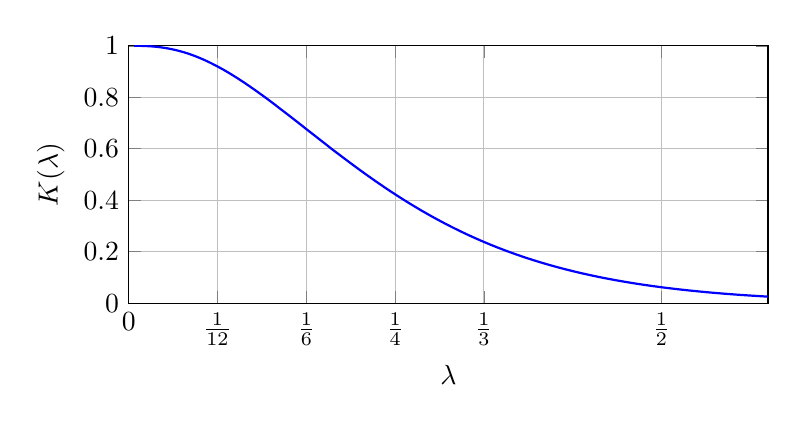
\begin{tikzpicture}
\begin{axis}[
    xlabel={$\lambda$},
    ylabel={$K(\lambda)$},
    ymin=0, ymax=1,
    xmin=0, xmax=0.6,
    xtick={0, 1/12, 1/6, 1/4, 1/3, 1/2},
    xticklabels={$0$, $\frac{1}{12}$, $\frac{1}{6}$, $\frac{1}{4}$, $\frac{1}{3}$, $\frac{1}{2}$},
    grid=major,
    width=0.8\textwidth,
    height=0.4\textwidth,
    samples=100,
    domain=0.005:0.6
]
\addplot[blue, thick, smooth] {exp(-12*x) * (1 + 12*x + (12*x)^2 / 2)};
\end{axis}
\end{tikzpicture}
\caption{Graph of $K(\lambda)$. (Note that $\lambda = 0$ is not included in the graph.)}
\end{figure}

The size of the test is $\underset{\lambda \in \Omega_0}{\max} K(\lambda) = K(1/2) = 0.0620$.

\mysectionstar{Q6}
Answer the following two questions under the assumption of normal populations with equal variances.

\mysubsectionstar{(i)}
The following are the numbers of sales which a random sample of nine salesmen of industrial chemicals in California and a random sample of six salesmen of industrial chemicals in Oregon made over a fixed period of time:
\[ \text{(California)} \quad x_i : 40, 46, 61, 38, 55, 63, 36, 60, 51 \]
\[ \text{(Oregon)} \quad y_i : 33, 62, 44, 54, 23, 42 \]
Using a 5\% level of significance, test whether or not Californian salesmen are more efficient in general. Write down the null and alternative hypothesis first.

$\newline$
Denote $X \sim N(\mu_1, \sigma^2)$ and $Y \sim N(\mu_2, \sigma^2)$, where $X$ and $Y$ are the number of sales made by Californian and Oregonian salesmen, respectively. \\
The null hypothesis is $H_0 : \mu_1 \leq \mu_2$ and the alternative hypothesis is $H_1 : \mu_1 > \mu_2$. \\
Note that, $\bar{x} = \frac{40 + 46 + 61 + 38 + 55 + 63 + 36 + 60 + 51}{9} = 50$ and $\bar{y} = \frac{33 + 62 + 44 + 54 + 23 + 42}{6} = 43$. \\
The sample variances are $s_x^2 = \frac{1}{8} \sum_{i=1}^{9} (x_i - 50)^2 = \frac{872}{8} = 109$ and $s_y^2 = \frac{1}{5} \sum_{i=1}^{6} (y_i - 43)^2 = \frac{984}{5} = 196.8$. \\
The pooled variance is $s_p^2 = \frac{(n-1)s_x^2 + (m-1)s_y^2}{n+m-2} = \frac{8 \cdot 109 + 5 \cdot 196.8}{9 + 6 - 2} = \frac{1856}{13}$, $s_p = \sqrt{\frac{1856}{13}}$. \\
For two unknown but equal variances and testing for difference in means, we use t distribution. \\
The test statistics is:
\[
W = \frac{\bar{x} - \bar{y}}{S_p \sqrt{\frac{1}{n} + \frac{1}{m}}}
\]
The rejection region is:
\begin{align*}
\{\bar{x} - \bar{y} > t_{\alpha, n+m-2} S_p \sqrt{\frac{1}{n} + \frac{1}{m}}\} &= \{\bar{x} - \bar{y} > t_{0.05, 13} \sqrt{\frac{1856}{13}(\frac{1}{9} + \frac{1}{6})}\} \\
&= \{\bar{x} - \bar{y} > 1.771 \sqrt{\frac{4640}{117}}\} \\
&= \{\bar{x} - \bar{y} > 11.15282\}
\end{align*}
From the sample, $\bar{x} - \bar{y} = 50 - 43 = 7$. Since $7 \nless 11.15282$, we fail to reject the null hypothesis. \\
Therefore, there is no evidence to suggest that Californian salesmen are more efficient in general.

\mysubsectionstar{(ii)}
Suppose that we wish to investigate whether males and females earn comparable wages in a certain industry. Sample data show that 14 randomly surveyed males earn on the average $213.5$ per week with a standard deviation of $16.5$, while 18 randomly surveyed females earn on the average $194.1$ per week with a standard deviation of $18.0$. Let $\mu_1$ denote the average wage of males and $\mu_2$ the average of females. Using a 5\% level of significance, test the null hypothesis that $\mu_1 = \mu_2$ against the alternative that $\mu_1 > \mu_2$.

$\newline$
$H_0 : \mu_1 = \mu_2$ and $H_1 : \mu_1 > \mu_2$. \\
Given $n = 14$, $m = 18$, $\bar{x} = 213.5$, $\bar{y} = 194.1$, $s_x = 16.5$, $s_y = 18.0$, $\alpha = 0.05$. \\
The pooled variance is $s_p^2 = \frac{(n-1)s_x^2 + (m-1)s_y^2}{n+m-2} = \frac{13 \cdot 16.5^2 + 17 \cdot 18.0^2}{30} = \frac{12063}{40}$, $s_p = \sqrt{\frac{12063}{40}}$. \\
The test statistics is:
\begin{align*}
W &= \frac{\bar{x} - \bar{y}}{S_p \sqrt{\frac{1}{n} + \frac{1}{m}}} = \frac{213.5 - 194.1}{\sqrt{\frac{12063}{40}} \sqrt{\frac{1}{14} + \frac{1}{18}}} = \frac{19.4}{\sqrt{\frac{12063}{40}} \sqrt{\frac{8}{63}}} = 3.134940792
\end{align*}
The rejection region is:
\[
W \geq t_{0.05, 30} = 1.697
\]
Since $3.134940792 \geq 1.697$, we reject the null hypothesis. \\
Therefore, there is evidence to suggest that male tend to earn more than females in that industry.


\mysectionstar{Q7}
Management training programs are often instituted to teach supervisory skills and thereby increase productivity. Suppose a company psychologist administers a set of examinations to each of 10 supervisors before such a training program begins and then administers similar examinations at the end of the program. The examinations are designed to measure supervisory skills, with higher scores indicating increased skill. The results of the tests are shown below:
\[
\begin{array}{c|cc}
\text{Supervisor} & \text{Pre-Test} & \text{Post-Test} \\
\hline
1 & 63 & 78 \\
2 & 93 & 92 \\
3 & 84 & 91 \\
4 & 72 & 80 \\
5 & 65 & 69 \\
6 & 72 & 85 \\
7 & 91 & 99 \\
8 & 84 & 82 \\
9 & 71 & 81 \\
10 & 80 & 87 \\
\end{array}
\]
Do the data provide evidence that the training program is effective in increasing supervisory skills, as measured by the examination scores? Set up the appropriate hypotheses and test them at 5\% significance level. State the assumptions made.

$\newline$
Denote $O_i$ be the $i-th$ supervisor pre-test score, $E_i$ be the $i-th$ supervisor post-test score, and $D_i = E_i - O_i$ be the difference in scores. \\
Set the null hypothesis be $H_0 : \mu_D = 0$, the training program is ineffective, and the alternative hypothesis be $H_1 : \mu_D > 0$, the training program is effective.
\[
\begin{array}{c|ccc}
\text{Supervisor} & O_i & E_i & D_i \\
\hline
1 & 63 & 78 & 15 \\
2 & 93 & 92 & -1 \\
3 & 84 & 91 & 7 \\
4 & 72 & 80 & 8 \\
5 & 65 & 69 & 4 \\
6 & 72 & 85 & 13 \\
7 & 91 & 99 & 8 \\
8 & 84 & 82 & -2 \\
9 & 71 & 81 & 10 \\
10 & 80 & 87 & 7 \\
\hline
\text{Total} & & & 69 \\
\text{Average} & & & 6.9 \\
\end{array}
\]
Assume $D_i \sim N(\mu_D, \sigma^2)$, where $\mu_D$ is the mean difference in scores. \\
The sample mean and variance of the differences are $\bar{D} = \frac{1}{10} \sum_{i=1}^{10} D_i = 6.9$ and $s_D^2 = \frac{1}{9} \sum_{i=1}^{10} (D_i - 6.9)^2 = \frac{883}{30}$, $s_D = \sqrt{\frac{883}{30}} = 5.42525$. \\
The test statistics for unknown but equal variances is:
\[
T = \frac{\bar{D}}{s_D / \sqrt{n-1}} \sim t_{n-1}
\]
For $\alpha = 0.05$, $n = 10$, $t_{0.05, 9} = 1.833$.
\[
T = \frac{6.9}{5.42525 / \sqrt{9}} = \frac{6.9}{5.42525 / 3} = 3.8155
\]
Since $3.8155 > 1.833$, we reject the null hypothesis at 5\% significance level. \\
Therefore, there is evidence to suggest that the training program is effective in increasing supervisory skills.

\newpage

\mysectionstar{Q8}
Let $X$ and $Y$ be the times in days required for maturation of Guardiola seeds from narrow-leaved and broad-leaved parents, respectively. Assume that both $X$ and $Y$ are distributed as normal and they are independent to each other. A sample of size 13 yields $s_X^2 = 9.88$ and the other sample of size 9 yields $s_Y^2 = 4.08$. \\
Test the hypothesis that the population variances of $X$ and $Y$ are equal. Use $\alpha = 0.05$.

$\newline$
Assume that $X \sim N(\mu_X, \sigma_X^2)$ and $Y \sim N(\mu_Y, \sigma_Y^2)$. \\
Let $H_0: \sigma_X^2 = \sigma_Y^2$ and $H_1: \sigma_X^2 \neq \sigma_Y^2$. \\
The test statistics for testing equality of variances is:
\[
W = \frac{n_X(n_Y - 1)s_X^2}{n_Y(n_X - 1)s_Y^2} \sim F_{n_X - 1, n_Y - 1}
\]
Because $H_1$ is two-sided, we consider two-tailed test: $F_{0.025, 12, 8} = 0.28476$ and $F_{0.975, 12, 8} = 4.19967$. \\
The rejection region is:
\[
\{W < 0.28476\} \cup \{W > 4.19967\}
\]
Since $W = \frac{13(9 - 1)9.88}{9(13 - 1)4.08} = 2.33188$, $0.28476 < 2.33188 < 4.19967$. \\
Therefore, we fail to reject the null hypothesis. \\
There is no evidence to suggest that the population variances of $X$ and $Y$ are different.
\end{document}
